
\begin{frame}
		\frametitle{Parallel Sort}
		\begin{figure}
				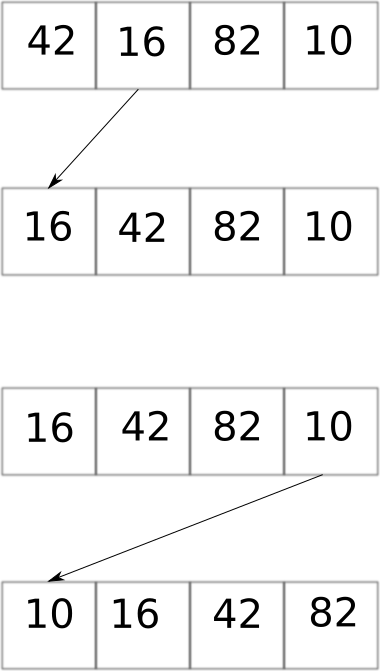
\includegraphics[width=0.3\linewidth]{figures/diagrams/sort/serialsort}
		\end{figure}	
\end{frame}

\begin{frame}
		\frametitle{Parallel Sort}
		\begin{figure}
				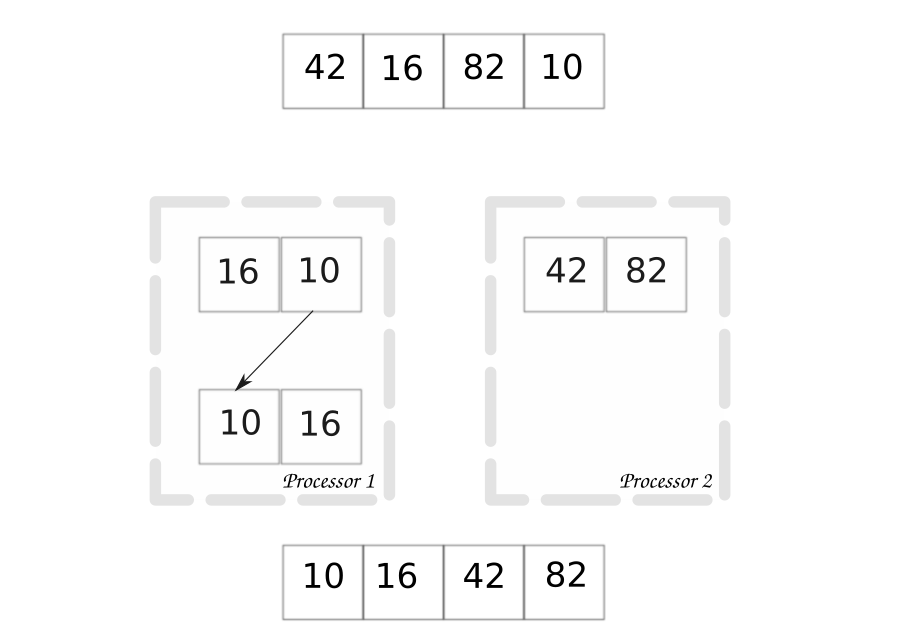
\includegraphics[width=0.8\linewidth]{figures/diagrams/sort/parallelsort}
		\end{figure}	
\end{frame}

\begin{frame}
		CLI examples of parallel utilities
\end{frame}


\begin{frame}[fragile]
		\frametitle{R parallel package}
		\center
		\begin{verbatim}
			library(doParallel)
			cl <- makeCluster(2)
			registerDoParallel(cl)
			foreach(i=1:3) %dopar% sqrt(i)
		\end{verbatim}
\end{frame}

\begin{frame}
		observed/expected speedup (figure)
\end{frame}

\begin{frame}
		\frametitle{Amdahl's law}
		\begin{figure}
				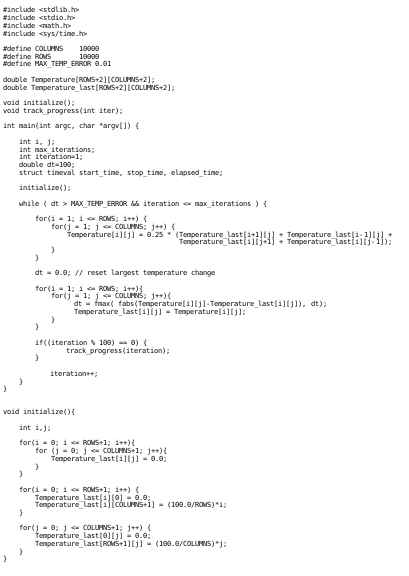
\includegraphics[width=0.4\linewidth]{figures/diagrams/amdahl/code}
		\end{figure}
\end{frame}

\begin{frame}
		\frametitle{Amdahl's law}
		\begin{figure}
				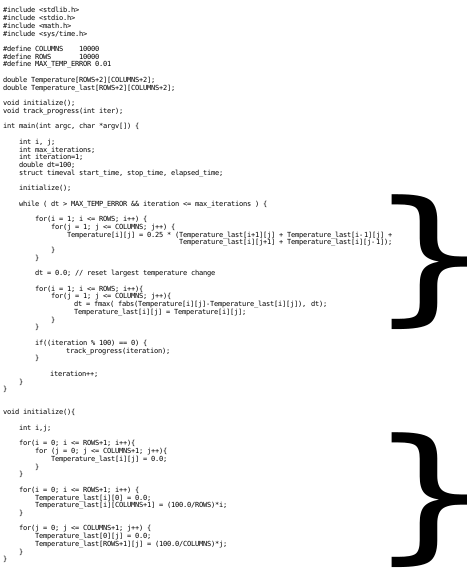
\includegraphics[width=0.4\linewidth]{figures/diagrams/amdahl/parallelblocks}
		\end{figure}
\end{frame}

\begin{frame}
		\frametitle{Amdahl's law}
		72 total lines of code \newline
		24 parallelizable lines of code\newline

		\color{red}34\% highest possible reduction of time!
\end{frame}

\begin{frame}
		\frametitle{Parallel Overhead}
		\begin{figure}
				\includegraphics[width=0.4\linewidth]{figures/diagrams/amdahl/overhead}
		\end{figure}
\end{frame}

\begin{frame}
		\frametitle{Parallel Overhead}
		\sout{34\% highest possible reduction of time!}\newline

		\color{red}Due to parallelization overhead, theorectical limit isn't
even possible.
\end{frame}

